\begin{textbox}{\href{https://compneuro.neuromatch.io/tutorials/W1D1_ModelTypes/student/W1D1_Tutorial1.html}{"What" models } }
\begin{subbox}{subbox}{Overview}
\scriptsize
We will explore \textbf{"What"} models, used to describe the data. To understand what our data looks like, we will visualize it in different ways. Then we will compare it to simple mathematical models. Specifically, we will:
\begin{itemize}
    \item 
Use spiking activity from hundreds of neurons and understand how it is organized
\item Visualize characteristics of the spiking activity across the population
\item Compute the distribution of "inter-spike intervals" (ISIs) for a single neuron
\item Consider several formal models of this distribution's shape and fit them to the data "by hand"
\end{itemize}

\end{subbox}

\begin{subbox}{subbox}{Exploring the Steinmetz dataset}
\scriptsize

We consider a subset of data from a study of \href{https://www.nature.com/articles/s41586-019-1787-x}{Steinmetz et al. (2019)}. In this study, Neuropixels probes were implanted in the brains of mice. Electrical potentials were measured by hundreds of electrodes along the length of each probe. Each electrode's measurements captured local variations in the electric field due to nearby spiking neurons. A spike sorting algorithm was used to infer spike times and cluster spikes according to common origin: a single cluster of sorted spikes is causally attributed to a single neuron.

In particular, a single recording session of spike times and neuron assignments was loaded and assigned to \textit{spike times} in the preceding setup.
Typically a dataset comes with some information about its structure. However, this information may be incomplete.

You might also apply some transformations or "pre-processing" to create a working representation of the data of interest, which might go partly undocumented depending on the circumstances. In any case it is important to be able to use the available tools to investigate unfamiliar aspects of a data structure.

\end{subbox}




\end{textbox}
%%%%%%%%%%%%%%%%%%%%%%%%%%%%%%%%%%%%%%%%%%%%%%%%%%
%%%%%%%%%%%%%%%%%%%%%%%%%%%%%%%%%%%%%%%%%%%%%%%%%%
\begin{textbox}{\href{https://compneuro.neuromatch.io/tutorials/W1D1_ModelTypes/student/W1D1_Tutorial1.html}{"What" models } }
\begin{subbox}{subbox}{Plotting total spike counts}
\scriptsize

The number of spikes over the entire recording is variable between neurons. More generally, some neurons tend to spike more than others in a given period. Let's explore what the distribution of spiking looks like across all the neurons in the dataset.

The plot shows that the majority of neurons are relatively "quiet" compared to the mean, while a small number of neurons are exceptionally "loud": they must have spiked more often to reach a large count.
If the mean neuron is more active than 68\% of the population, what does that imply about the relationship between the mean neuron and the median (50th percentile) neuron?

\centering
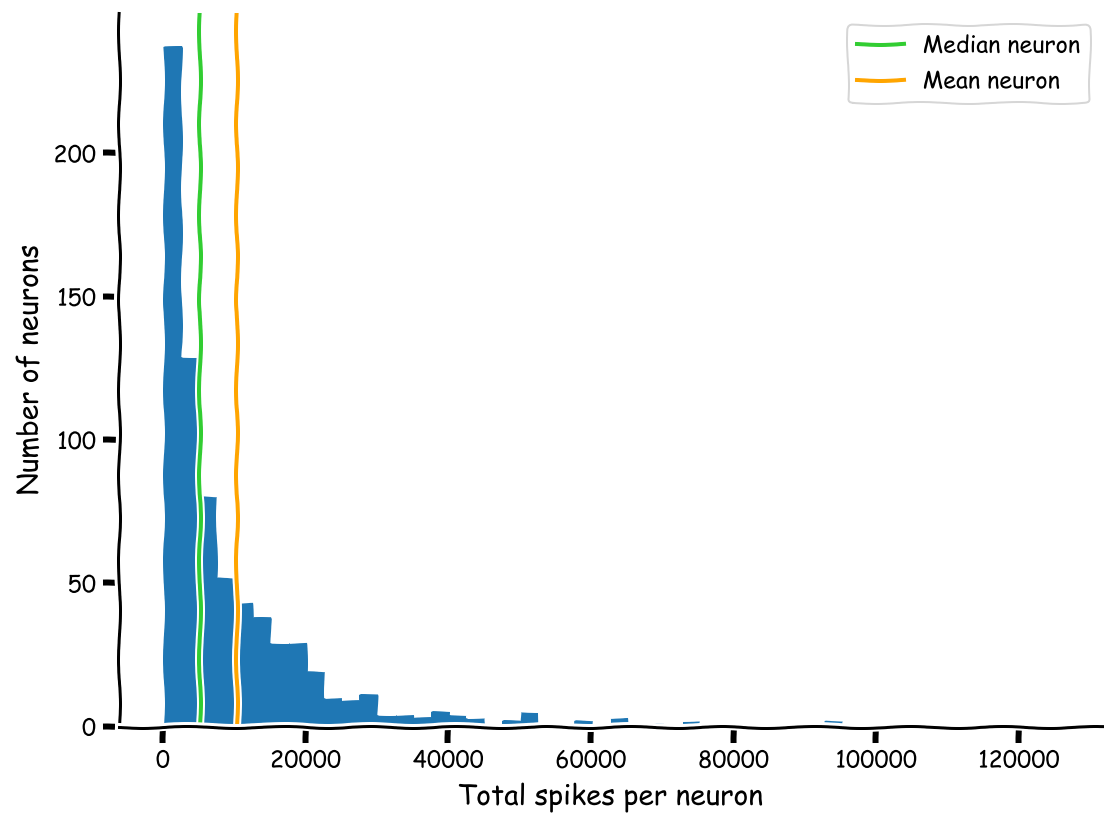
\includegraphics[scale=0.11]{Figures/MT/MT_Figure1.png}
\end{subbox}


\begin{subbox}{subbox}{Visualizing neuronal spiking activity}
\scriptsize

A "raster" plot, where the spikes from each neuron appear in a different row.

Plotting a large number of neurons can give you a sense for the characteristics in the population. 

\centering
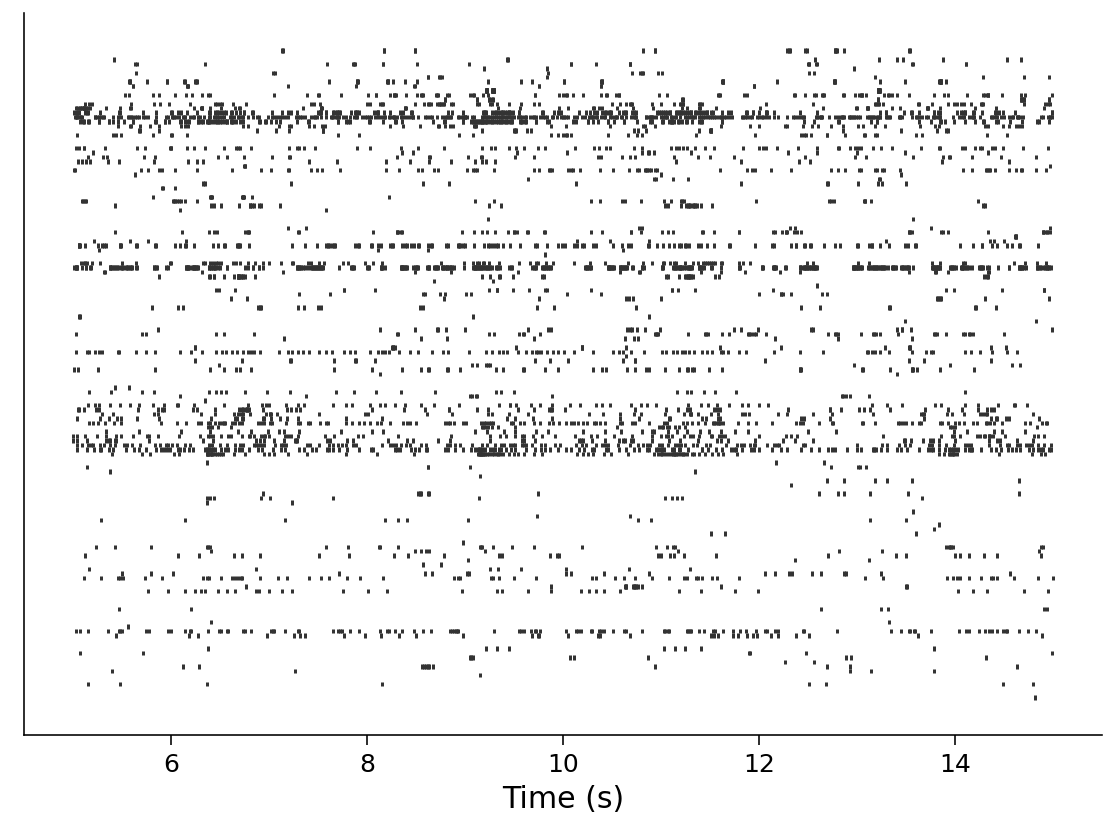
\includegraphics[scale=0.3]{Figures/MT/MT_Figure2.png}
\end{subbox}
\end{textbox}
%%%%%%%%%%%%%%%%%%%%%%%%%%%%%%%%%%%%%%%%%%%%%%%%%%
%%%%%%%%%%%%%%%%%%%%%%%%%%%%%%%%%%%%%%%%%%%%%%%%%%
\begin{textbox}{\href{https://compneuro.neuromatch.io/tutorials/W1D1_ModelTypes/student/W1D1_Tutorial1.html}{"What" models }   }
\begin{subbox}{subbox}{Inter-spike intervals and their distributions}
\scriptsize

Given the ordered arrays of spike times, what can we ask next?

Scientific questions are informed by existing models. So, what knowledge do we already have that can inform questions about this data?

We know that there are physical constraints on neuron spiking. Spiking costs energy, which the neuron's cellular machinery can only obtain at a finite rate. Therefore neurons should have a refractory period: they can only fire as quickly as their metabolic processes can support, and there is a minimum delay between consecutive spikes of the same neuron.
More generally, we can ask "how long does a neuron wait to spike again?" or "what is the longest a neuron will wait?" Can we transform spike times into something else, to address questions like these more directly?
We can consider the inter-spike times (or interspike intervals: ISIs). These are simply the time differences between consecutive spikes of the same neuron.
In general, the shorter ISIs are predominant, with counts decreasing rapidly (and smoothly, more or less) with increasing ISI. However, counts also rapidly decrease to zero with decreasing ISI below the maximum of the distribution (8-11 ms). The absence of these very low ISIs agrees with the refractory period hypothesis: the neuron cannot fire quickly enough to populate this region of the ISI distribution.

\end{subbox}
\begin{subbox}{subbox}{What is the functional form of an ISI distribution?}
\scriptsize


The ISI histograms seem to follow continuous, monotonically decreasing functions above their maxima. The function is clearly non-linear. Could it belong to a single family of functions?

To motivate the idea of using a mathematical function to explain physiological phenomena, let's define a few different function forms that we might expect the relationship to follow: exponential, inverse, and linear.

\begin{center}
    
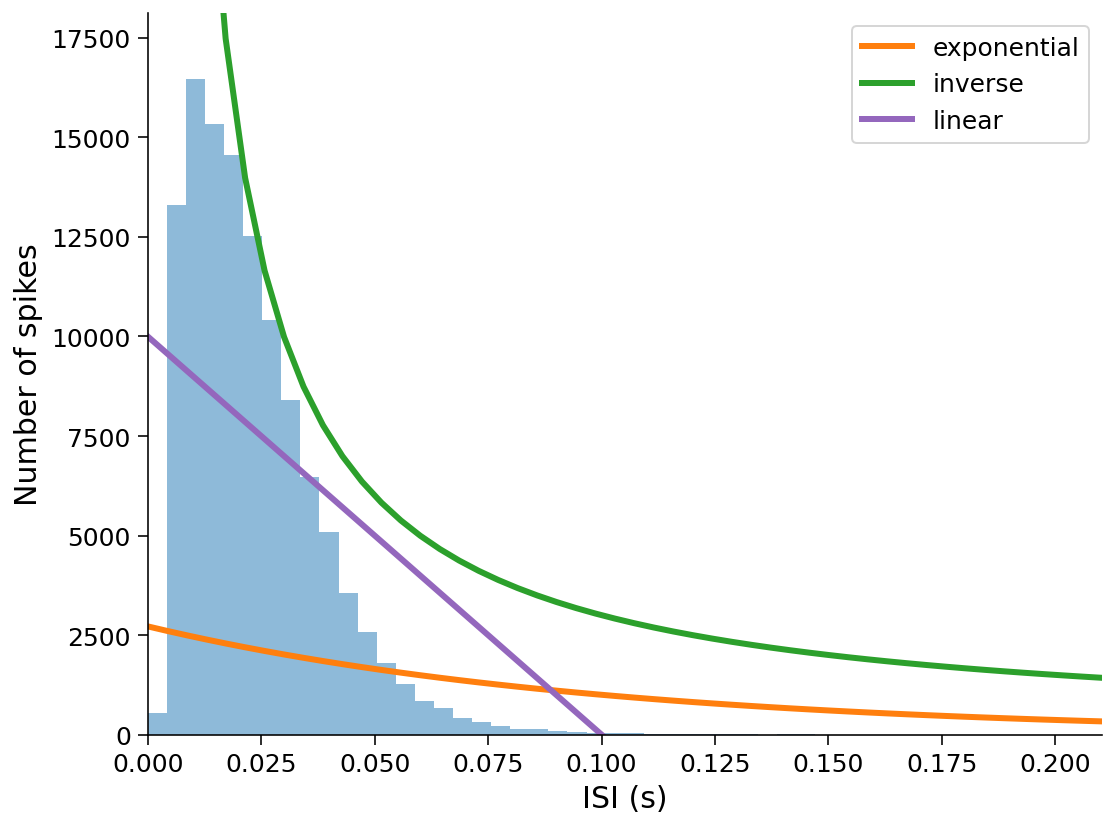
\includegraphics[scale=0.15]{Figures/MT/MT_Figure4.png}
\end{center}
The exponential function can be made to fit the data much better than the linear
or inverse function.
\end{subbox}
\end{textbox}
%%%%%%%%%%%%%%%%%%%%%%%%%%%%%%%%%%%%%%%%%%%%%%%%%%
%%%%%%%%%%%%%%%%%%%%%%%%%%%%%%%%%%%%%%%%%%%%%%%%%%
%%%TUTORIAL 2
%%%%%%%%%%%%%%%%%%%%%%%%%%%%%%%%%%%%%%%%%%%%%%%%%%
%%%%%%%%%%%%%%%%%%%%%%%%%%%%%%%%%%%%%%%%%%%%%%%%%%
\begin{textbox}{\href{https://compneuro.neuromatch.io/tutorials/W1D1_ModelTypes/student/W1D1_Tutorial2.html}{"How" models } }
\begin{subbox}{subbox}{Overview }
\scriptsize
We will explore models that can potentially explain \textbf{"How"} the spiking data we have observed is produced. To understand the mechanisms  we will build simple neuronal models and compare their spiking response to real data. We will:
\begin{enumerate}
    \item 
 Simulate a  simple "leaky integrate-and-fire" neuron model 
\item Make the model more complicated — but also more realistic—by adding more physiologically-inspired details
\end{enumerate}
\end{subbox}
\begin{subbox}{subbox}{How does a neuron spike? }
\scriptsize

A neuron charges and discharges an electric field across its cell membrane. The state of this electric field can be described by the \textit{membrane potential}. The membrane potential rises due to excitation of the neuron, and when it reaches a threshold a spike occurs. The potential resets, and must rise to a threshold again before the next spike occurs.

One of the simplest models of spiking neuron behavior is the linear integrate-and-fire (LIF) model neuron. In this model, the neuron increases its membrane potential $V_m$ over time in response to excitatory input currents $I$ scaled by some factor $\alpha$:
\begin{equation}
dV_m = {\alpha}I
\end{equation}
Once $V_m$ reaches a threshold value a spike is produced, $V_m$ is reset to a starting value, and the process continues. 

Here, we will take the starting and threshold potentials as $0$ and $1$, respectively. So, for example, if $\alpha I=0.1$ is constant---that is, the input current is constant---then $dV_m=0.1$, and at each timestep the membrane potential $V_m$ increases by $0.1$ until after $(1-0)/0.1 = 10$ timesteps it reaches the threshold and resets to $V_m=0$, and so on.

Note that we define the membrane potential $V_m$ as a scalar: a single real (or floating point) number. However, a biological neuron's membrane potential will not be exactly constant at all points on its cell membrane at a given time. We could capture this variation with a more complex model (e.g. with more numbers). Do we need to? 

The proposed model is a 1D simplification. There are many details we could add to it, to preserve different parts of the complex structure and dynamics of a real neuron. If we were interested in small or local changes in the membrane potential, our 1D simplification could be a problem. However, we'll assume an idealized "point" neuron model for our current purpose.
\begin{center}
    
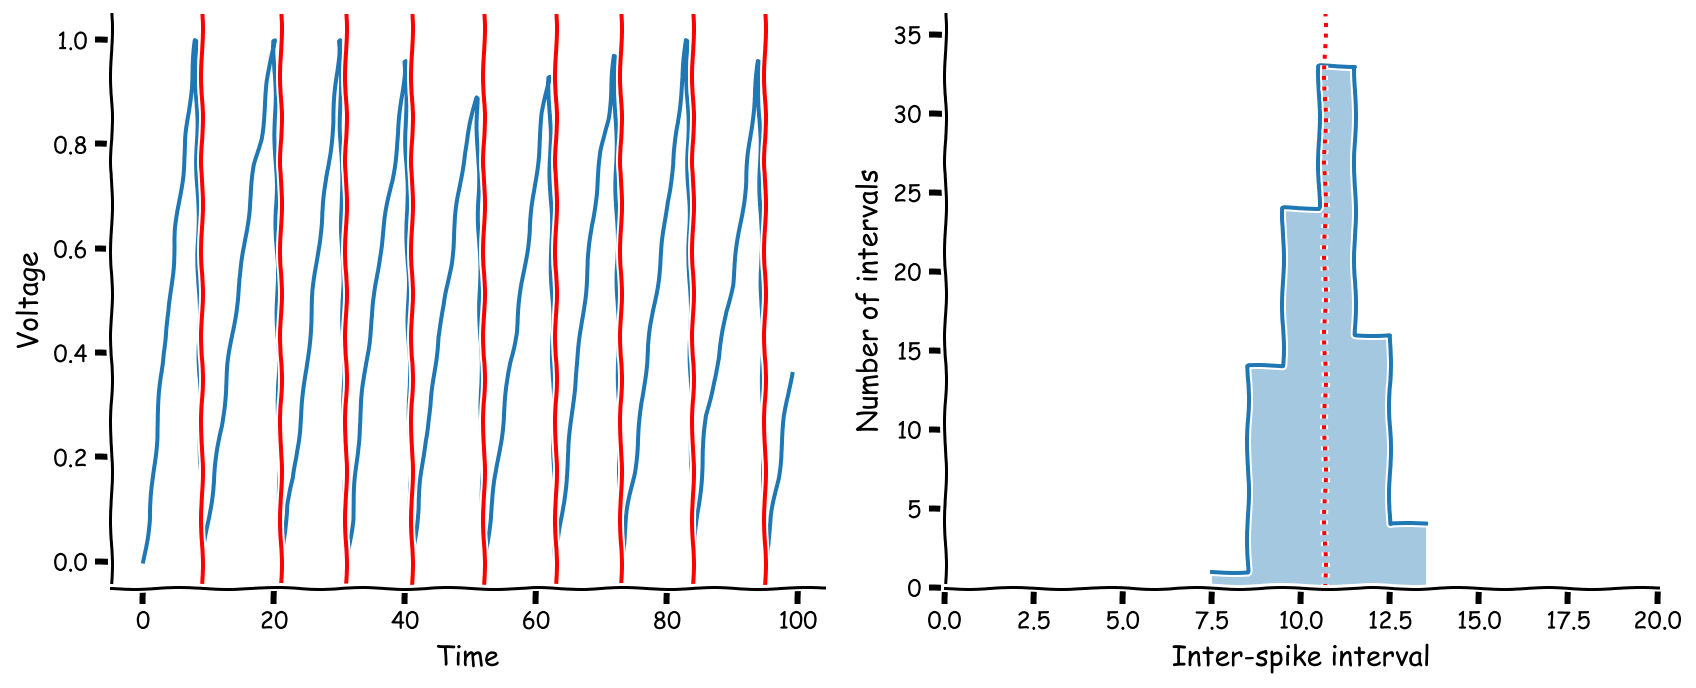
\includegraphics[scale=0.08]{Figures/MT/MT_Figure5.png}
\end{center}
\end{subbox}
\end{textbox}
%%%%%%%%%%%%%%%%%%%%%%%%%%%%%%%%%%%%%%%%%%%%%%%%%%
%%%%%%%%%%%%%%%%%%%%%%%%%%%%%%%%%%%%%%%%%%%%%%%%%%
\begin{textbox}{\href{https://compneuro.neuromatch.io/tutorials/W1D1_ModelTypes/student/W1D1_Tutorial2.html}{"How" models } }

\begin{subbox}{subbox}{Spiking Inputs}
\scriptsize

Given our simplified model for the neuron dynamics, we still need to consider what form the input $I$ will take. How should we specify the firing behavior of the presynaptic neuron(s) providing the inputs to our model neuron? 

Unlike in the simple example the input current is generally not constant. Physical inputs tend to vary with time. We can describe this variation with a distribution.

We'll assume the input current $I$ over a timestep is due to equal contributions from a non-negative ($\ge 0$) integer number of input spikes arriving in that timestep. Our model neuron might integrate currents from 3 input spikes in one timestep, and 7 spikes in the next timestep. We should see similar behavior when sampling from our distribution.

Given no other information about the input neurons, we will also assume that the distribution has a mean, and that the spiking events of the input neuron(s) are independent in time. Are these reasonable assumptions in the context of real neurons?

A suitable distribution given these assumptions is the Poisson distribution, which we'll use to model $I$:

\begin{equation}
I \sim \mathrm{Poisson}(\lambda)
\end{equation}

where $\lambda$ is the mean of the distribution: the average rate of spikes received per timestep.

\end{subbox}
\begin{subbox}{subbox}{Inhibitory signals}
\scriptsize

Our linear IF neuron from the previous section was indeed able to produce spikes. However, our ISI histogram doesn't look much like an empirical ISI histograms, which has an exponential-like shape. What is our model neuron missing, given that it doesn't behave like a real neuron?

In the previous model we only considered excitatory behavior. We know, however, that there are other factors that can drive $V_m$ down. First is the natural tendency of the neuron to return to some steady state or resting potential. We can update our previous model as follows:

\begin{equation}
dV_m = -{\beta}V_m + {\alpha}I
\end{equation}

where $V_m$ is the current membrane potential and $\beta$ is some leakage factor. This is a basic form of the popular LIF model.

We also know that in addition to excitatory presynaptic neurons, we can have inhibitory presynaptic neurons as well. We can model these inhibitory neurons with another Poisson random variable:
\begin{align}
I &= I_{\mathrm{exc}} - I_{\mathrm{inh}} \\
I_{\mathrm{exc}} &\sim \mathrm{Poisson}(\lambda_{\mathrm{exc}}) \\
I_{\mathrm{inh}} &\sim \mathrm{Poisson}(\lambda_{\mathrm{inh}})
\end{align}

where $\lambda_{\mathrm{exc}}$ and $\lambda_{\mathrm{inh}}$ are the average spike rates (per timestep) of the excitatory and inhibitory presynaptic neurons, respectively.

\end{subbox}
\end{textbox}
%%%%%%%%%%%%%%%%%%%%%%%%%%%%%%%%%%%%%%%%%%%%%%%%%%
%%%%%%%%%%%%%%%%%%%%%%%%%%%%%%%%%%%%%%%%%%%%%%%%%%
\begin{textbox}{\href{https://compneuro.neuromatch.io/tutorials/W1D1_ModelTypes/student/W1D1_Tutorial2.html}{"How" models } }

\begin{subbox}{subbox}{LIF + inhibition neuron}
\scriptsize

\begin{enumerate}
    \item 
Raising the excitatory rate while keeping inhibitory rate the same results in
more frequent firing and shorter ISIs. This makes intuitive sense - more excitatory input
means higher responses.
\item Raising the inhibitory rate while keeping the excitatory rate the same results
in less frequent firing and longer ISIs. This makes intuitive sense - more inhibitory input
means lower responses.
\item If the excitatory and inhibitory rates are equal, the average inter-spike interval
stays the same even if you raise both. This is because they balance each other out.
\item Yes, these ISIs look more exponential, like what we observed.
\end{enumerate}

\begin{center}
    
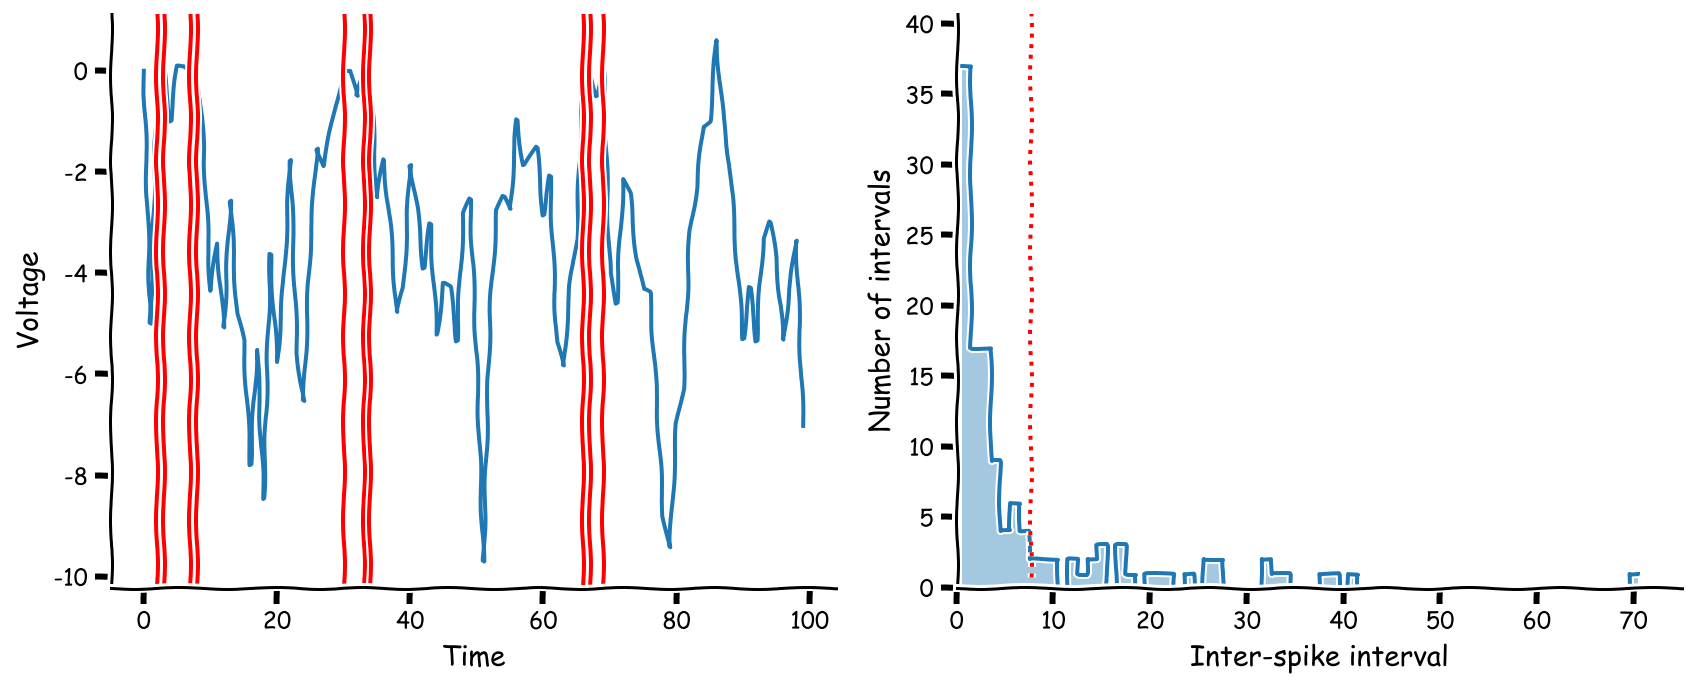
\includegraphics[scale=0.1]{Figures/MT/MT_Figure6.png}
\end{center}

\end{subbox}
\begin{subbox}{subbox}{Notation}
\scriptsize
\begin{align*}
V_m &\quad \text{membrane potential} \\
dV_m &\quad \text{change in membrane potential}\\
C_m &\quad \text{membrane capacitance}\\
I &\quad \text{input current}\\
R_m &\quad \text{membrane resistance}:\\
V_\mathrm{rest} &\quad \text{resting potential}\\
\alpha &\quad \text{scaling factor for input current}\\
\beta &\quad \text{leakage factor}\\
\lambda &\quad \text{average spike rate}\\
\lambda_\mathrm{exc} &\quad \text{average spike rate for excitatory neurons}\\
\lambda_\mathrm{inh} &\quad \text{average spike rate for inhibitory neurons}\\
\end{align*}
\end{subbox}
\end{textbox}
%%%%%%%%%%%%%%%%%%%%%%%%%%%%%%%%%%%%%%%%%%%%%%%%%%
%%%%%%%%%%%%%%%%%%%%%%%%%%%%%%%%%%%%%%%%%%%%%%%%%%
%%%%% TUTORIAL 3
%%%%%%%%%%%%%%%%%%%%%%%%%%%%%%%%%%%%%%%%%%%%%%%%%%
%%%%%%%%%%%%%%%%%%%%%%%%%%%%%%%%%%%%%%%%%%%%%%%%%%
\begin{textbox}{\href{https://compneuro.neuromatch.io/tutorials/W1D1_ModelTypes/student/W1D1_Tutorial3.html}{"Why" models }  }

\begin{subbox}{subbox}{Overview}
\scriptsize
We will explore models and techniques that can potentially explain \textbf{why} the spiking data we have observed is produced the way it is.

To understand why different spiking behaviors may be beneficial, we will learn about the concept of entropy. Specifically, we will:

\begin{enumerate}
    \item  Write code to compute formula for entropy, a measure of information
 \item  Compute the entropy of a number of toy distributions
 \item  Compute the entropy of spiking activity from the Steinmetz dataset

\end{enumerate}
\end{subbox}
\begin{subbox}{subbox}{Optimization and Information}
\scriptsize
Neurons can only fire so often in a fixed period of time, as the act of emitting a spike consumes energy that is depleted and must eventually be replenished. To communicate effectively for downstream computation, the neuron would need to make good use of its limited spiking capability. This becomes an optimization problem: 

What is the optimal way for a neuron to fire in order to maximize its ability to communicate information?

In order to explore this question, we first need to have a quantifiable measure for information. Shannon introduced the concept of entropy to do just that, and defined it as

\begin{equation}
H_b(X) = -\sum_{x\in X} p(x) \log_b p(x)
\end{equation}

where $H$ is entropy measured in units of base $b$ and $p(x)$ is the probability of observing the event $x$ from the set of all possible events in $X$. See the Bonus Section 1 for a more detailed look at how this equation was derived.

The most common base of measuring entropy is $b=2$, so we often talk about \textbf{bits} of information, though other bases are used as well (e.g. when $b=e$ we call the units \textit{nats}).

A distribution with mass split equally between two points looks like:

\begin{center}
    
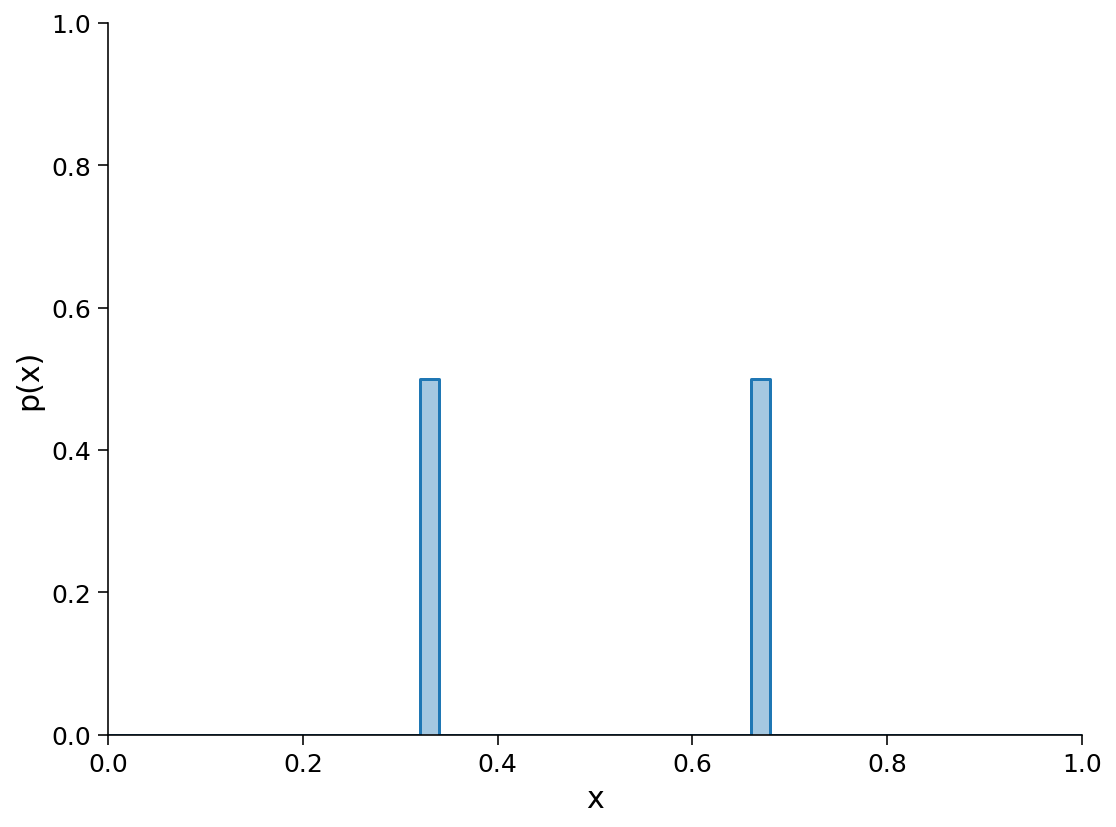
\includegraphics[scale=0.2]{Figures/MT/MT_Figure7.png}
\end{center}

Here, the entropy calculation is: $-(0.5 \log_2 0.5 + 0.5\log_2 0.5)=1$
ere is 1 bit of entropy. This means that before we take a random sample, there is 1 bit of uncertainty about which point in the distribution the sample will fall on: it will either be the first peak or the second one. 

\end{subbox}
\end{textbox}
%%%%%%%%%%%%%%%%%%%%%%%%%%%%%%%%%%%%%%%%%%%%%%%%%%
%%%%%%%%%%%%%%%%%%%%%%%%%%%%%%%%%%%%%%%%%%%%%%%%%%
\begin{textbox}{\href{https://compneuro.neuromatch.io/tutorials/W1D1_ModelTypes/student/W1D1_Tutorial3.html}{"Why" models } }


\begin{subbox}{subbox}{Entropy}
\scriptsize


Likewise, if we make one of the peaks taller and the other one shorter, the entropy will decrease because of the increased certainty that the sample will fall on one point and not the other: : $-(0.2 \log_2 0.2 + 0.8\log_2 0.8)\approx 0.72$

If we split the probability mass among even more points, the entropy continues to increase. Let's derive the general form for $N$ points of equal mass, where $p_i=p=1/N$:

\begin{align}
-\sum_i p_i \log_b p_i &= -\sum_i^N \frac{1}{N} \log_b \frac{1}{N} \\
&= -\log_b \frac{1}{N} \\
&= \log_b N
\end{align}

If we have $N$ discrete points, the \textit{uniform distribution} (where all points have equal mass) is the distribution with the highest entropy: $\log_b N$. This upper bound on entropy is useful when considering binning strategies, as any estimate of entropy over $N$ discrete points (or bins) must be in the interval $[0, \log_b N]$

\end{subbox}

\begin{subbox}{subbox}{Information, neurons, and spikes}
\scriptsize
We'll consider three hypothetical neurons that all have the same mean ISI, but with different distributions:
\begin{enumerate}
\item Deterministic
\item Uniform
\item Exponential
\end{enumerate}
Fixing the mean of the ISI distribution is equivalent to fixing its inverse: the neuron's mean firing rate. If a neuron has a fixed energy budget and each of its spikes has the same energy cost, then by fixing the mean firing rate, we are normalizing for energy expenditure. This provides a basis for comparing the entropy of different ISI distributions. In other words: if our neuron has a fixed budget, what ISI distribution should it express (all else being equal) to maximize the information content of its outputs?

Let's construct our three distributions and see how their entropies differ.

\begin{center}
    
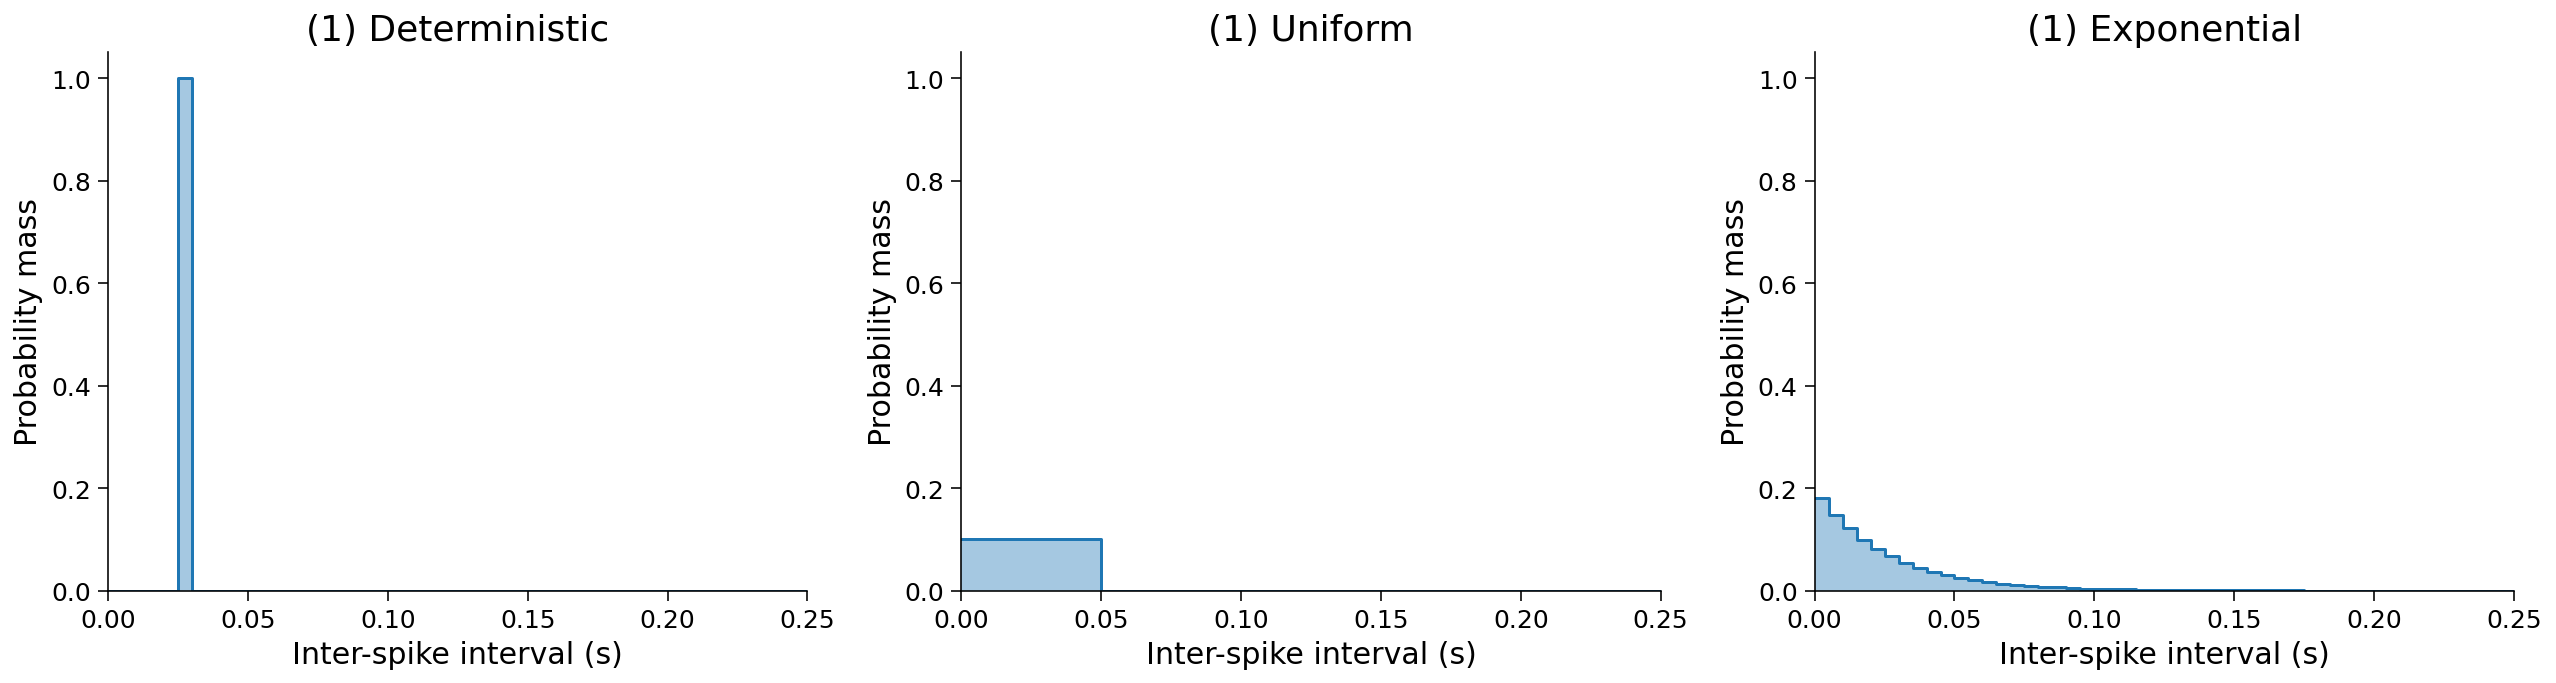
\includegraphics[scale=0.14]{Figures/MT/MT_Figure8.png}
\end{center}


\begin{enumerate}
\item Deterministic: 0.00 bits
\item Uniform: 3.32 bits
\item Exponential: 3.77 bits
\end{enumerate}
\end{subbox}

\end{textbox}
%%%%%%%%%%%%%%%%%%%%%%%%%%%%%%%%%%%%%%%%%%%%%%%%%%
%%%%%%%%%%%%%%%%%%%%%%%%%%%%%%%%%%%%%%%%%%%%%%%%%%
\begin{textbox}{\href{https://compneuro.neuromatch.io/tutorials/W1D1_ModelTypes/student/W1D1_Tutorial3.html}{"Why" models } }


\begin{subbox}{subbox}{Calculate entropy of ISI distributions from data
}
\scriptsize


In the previous example we created the PMFs by hand to illustrate idealized scenarios. How would we compute them from data recorded from actual neurons?

One way is to convert the ISI histograms we've previously computed into discrete probability distributions using the following equation:

\begin{equation}
p_i = \frac{n_i}{\sum\nolimits_{i}n_i}
\end{equation}

where $p_i$ is the probability of an ISI falling within a particular interval $i$ and $n_i$ is the count of how many ISIs were observed in that interval.

\begin{center}
    
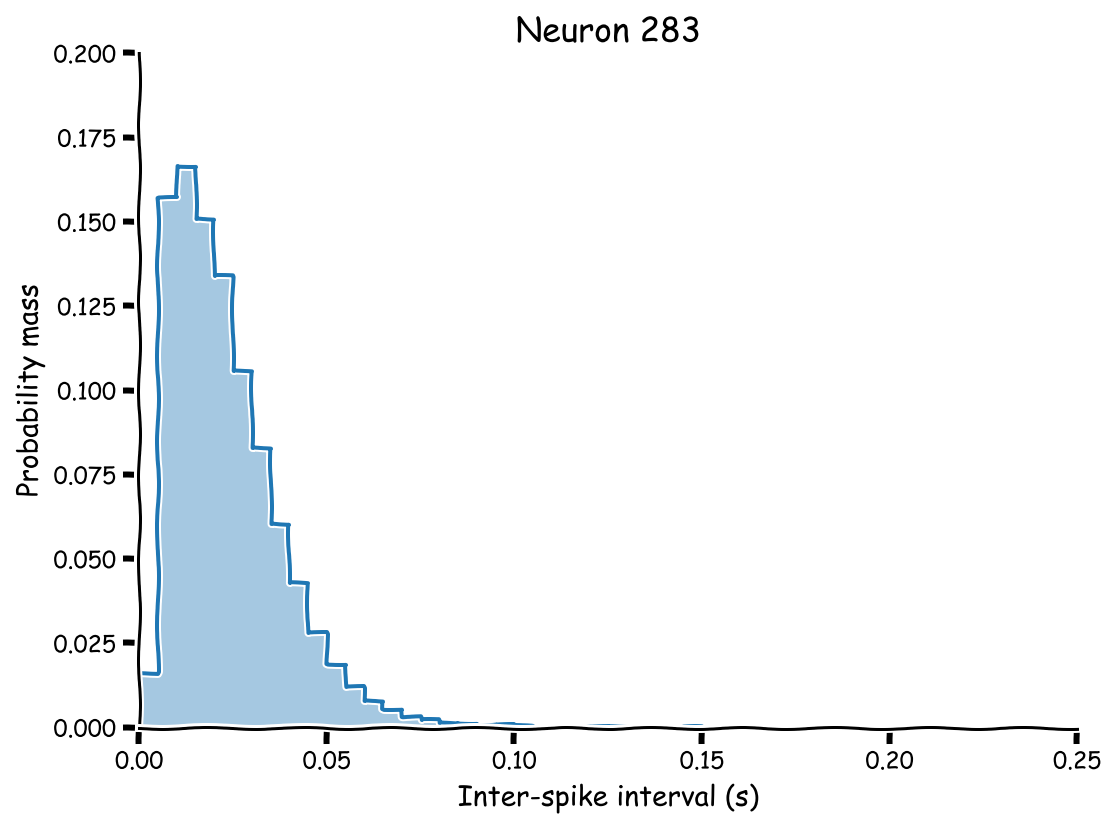
\includegraphics[scale=0.1]{Figures/MT/MT_Figure9.png}
\end{center}
Entropy for Neuron 283: 3.36 bits

\end{subbox}

\begin{subbox}{subbox}{Summary}
\scriptsize
We used different types of models to understand the spiking behavior of neurons recorded in the Steinmetz data set. 

\begin{itemize}
\item We used "what" models to discover that the ISI distribution of real neurons is closest to an exponential distribution
\item We used "how" models to discover that balanced excitatory and inhibitory inputs, coupled with a leaky membrane, can give rise to neuronal spiking with exhibiting such an exponential ISI distribution
 \item We used "why" models to discover that exponential ISI distributions contain the most information when the mean spiking is constrained
\end{itemize}
\end{subbox}

\begin{subbox}{subbox}{Notation}
\tiny
\begin{align*}
H(X) &\quad \text{entropy of random variable X}\\
b &\quad \text{base, e.g. b=2 or b=e}\\
x &\quad \text{event x}\\
p(x) &\quad \text{probability of observing event x}\\
\text{ISI} &\quad \text{interspike interval}\\
n_i &\quad \text{count of observed ISIs in interval i}\\
p_i  &\quad \text{probability of of an ISI falling within a particular interval i}
\end{align*}
\end{subbox}
\end{textbox}
